% Options for packages loaded elsewhere
\PassOptionsToPackage{unicode}{hyperref}
\PassOptionsToPackage{hyphens}{url}
%
\documentclass[
]{article}
\usepackage{lmodern}
\usepackage{amssymb,amsmath}
\usepackage{ifxetex,ifluatex}
\ifnum 0\ifxetex 1\fi\ifluatex 1\fi=0 % if pdftex
  \usepackage[T1]{fontenc}
  \usepackage[utf8]{inputenc}
  \usepackage{textcomp} % provide euro and other symbols
\else % if luatex or xetex
  \usepackage{unicode-math}
  \defaultfontfeatures{Scale=MatchLowercase}
  \defaultfontfeatures[\rmfamily]{Ligatures=TeX,Scale=1}
\fi
% Use upquote if available, for straight quotes in verbatim environments
\IfFileExists{upquote.sty}{\usepackage{upquote}}{}
\IfFileExists{microtype.sty}{% use microtype if available
  \usepackage[]{microtype}
  \UseMicrotypeSet[protrusion]{basicmath} % disable protrusion for tt fonts
}{}
\makeatletter
\@ifundefined{KOMAClassName}{% if non-KOMA class
  \IfFileExists{parskip.sty}{%
    \usepackage{parskip}
  }{% else
    \setlength{\parindent}{0pt}
    \setlength{\parskip}{6pt plus 2pt minus 1pt}}
}{% if KOMA class
  \KOMAoptions{parskip=half}}
\makeatother
\usepackage{xcolor}
\IfFileExists{xurl.sty}{\usepackage{xurl}}{} % add URL line breaks if available
\IfFileExists{bookmark.sty}{\usepackage{bookmark}}{\usepackage{hyperref}}
\hypersetup{
  hidelinks,
  pdfcreator={LaTeX via pandoc}}
\urlstyle{same} % disable monospaced font for URLs
\usepackage{graphicx}
\makeatletter
\def\maxwidth{\ifdim\Gin@nat@width>\linewidth\linewidth\else\Gin@nat@width\fi}
\def\maxheight{\ifdim\Gin@nat@height>\textheight\textheight\else\Gin@nat@height\fi}
\makeatother
% Scale images if necessary, so that they will not overflow the page
% margins by default, and it is still possible to overwrite the defaults
% using explicit options in \includegraphics[width, height, ...]{}
\setkeys{Gin}{width=\maxwidth,height=\maxheight,keepaspectratio}
% Set default figure placement to htbp
\makeatletter
\def\fps@figure{htbp}
\makeatother
\setlength{\emergencystretch}{3em} % prevent overfull lines
\providecommand{\tightlist}{%
  \setlength{\itemsep}{0pt}\setlength{\parskip}{0pt}}
\setcounter{secnumdepth}{-\maxdimen} % remove section numbering

\author{}
\date{}

\begin{document}

\begin{figure}
\centering
\includegraphics{img/cover.es.svg}
\caption{Cover}
\end{figure}

\hypertarget{luxe1zaro-strassenmagazin}{%
\subsection{Lázaro Strassenmagazin}\label{luxe1zaro-strassenmagazin}}

Ein OpenSource Magazin, für Obdachlose, von Obdachlosen. Lázaro findet
man im Internet unter fb.me/el.lazaro.periodico. Lázaro basiert 100\%
auf Voluntärarbeit. Dazu benötigen wir Artikel. Wenn Sie einen Artikel
schreiben möchten, posten Sie einfach auf der Facebook Seite einen
Beitrag und wir werden ihn, wenn er gut ist, veröffentlichen. Lázaro
kann vom Internet heruntergeladen und selber geruckt werden. Auf der
Webseite findet man dazu mehr Informationen. Lázaro ist auch eine gute
Möglichkeit für Kirchen oder Hilfswerke, die sich für Obdachlose
engagieren wollen, indem Sie dass Heft drucken lassen und den
Obdachlosen zum Selbstkostenpreis verkaufen, und somit eine
Verdienstmöglichkeit schaffen. Der Quellcode von Lázaro kann dabei
angepasst und falls gewünscht eigene Artikel eingebracht werden. Von den
Verkäufern wird erwartet, dass 10\% des Gewinns für einen guten Zweck
gespendet werden, dies ist jedoch nicht zwingend

\begin{figure}
\centering
\includegraphics{img/logo3.es.svg\#right}
\caption{Logo}
\end{figure}

\hypertarget{life-is-hard}{%
\subsection{Life is hard\ldots{}}\label{life-is-hard}}

In der Schweiz gibt es ja wenn es einem Langweilig ist viele
Möglichkeiten, sich abzulenken. Eine dieser vielen Möglichkeiten steht
zum Beispiel in Basel, die Mustermesse. Dort steht ja nun seit einigen
Jahren der Messeturm, ein schönes Hotel, in dem man, wenn man Geld hat,
ganz schön den Vergnügungen dieser Welt fröhnen kann. Wenn man nun schon
lange nicht mehr in der Schweiz war, denkt man sich, man möchte doch
einmal einen Blick über das nächtliche Basel werfen, von der
vielgerühmten Bar Rouge aus. Da man als HoPreBo1 Abends sowieso nichts
zu tun hat, versucht man einfach sein Glück, und geht durch den Eingang
und versucht möglichst wenig aufzufallen, weswegen man sich auch schnell
Richtung Lift begibt, um in diese Bar zu gelangen. Im Obersten Stock
hält dann der Lift, man steigt aus, und begibt sich zu dieser Bar.
Allerdings hat man dabei vergessen, dass wir uns in der Schweiz
befinden, denn am Eingang wird man darauf hingewiesen, dass der Zutritt
nur für VIP Gäste gestattet ist. Dafür wird man von einem Wunderschönen
Zitat von Friedrich Hölderlin beglückt welches dort von der Wand Prangt:
``Das Leben ist wie es ist, deshalb ist es so schön\ldots{}'' Naja, beim
Lesen solcher Zitate kommen mir immer noch andere Zitate in den Sinn,
wie z.B. ``Die Beine des Lahmen hängen schlaff herunter: so ist ein
weiser Spruch im Mund der Toren.'' In Nicaragua gibt es nicht wirklich
viele Bücher in denen man Zitate lesen könnte, bzw. die meisten Leute
haben einfach ein Büchergestell, in welches sie Bücher gestellt haben,
die einfach auf dem Bücherflohmark als Dekorationsgegenstand gekauft
worden sind, da man meistens gar kein Englisch versteht. Dafür gibt es
ganz schöne Zitate von wunderbaren Menschen, die dort einfach
herumlaufen. Einer davon ist z.B. mein Freund John Oliver. Er sitzt
immer in der Calle Cansada in Granada, und liest den Touristen Gedichte
vor oder verkauft kleines Kunsthandwerk, selber gemalte Bilder oder
sonstige Sachen. John Oliver hatte ein hartes Leben, er musste im
Bürgerkrieg kämpfen, wurde verwundet und musste aus dem Spital abhauen.
Er musste sich immer irgendwie durchschlagen. Später hat er dann auch
noch ein Bein verloren, und jetzt geht er immer an Krücken. Aber genauso
hart wie sein Leben auch war, so gross ist auch sein Herz. Als ich ihn
kennenlernte, fragte ich ihn, ob er Gospel singen könne, und er fing mit
rauher Stimme ein altes englisches Kirchenlied aus Bluefields zu Singen,
so dass es mich Schauderte. Leider kann ich jetzt hier keines seiner
Gedichte erzählen, weil zwischen uns eine halbe Weltkugel ist, und er
kein Telefon hat. Vielleicht im nächsten Heft. Ich war bis vor kurzem
noch in Ausschaffungshaft in Managua, und wusste nicht einmal, ob er
noch lebt, weil ich so lange in Haft war, und er kurz vorher Obdachlos
wurde, und viele der Jungs dort im Moment nicht genug zu Essen haben.

Aber neulich habe ich von ihm gehört, ich werde ihn also wieder
antreffen, wenn ich wieder nach Granada komme. Ab und zu haben wir
zusammen Strassenmusik gemacht, John Oliver hatte eine Aluminium-Pfanne
und hat percussion damit gespielt, und ich die Gittare. Einmal war eine
Französin aus der Bretagne zu besuch, so eine richtige Falbala, wie aus
dem Asterix-Band. Wir habe dann ein Lied von Jamaika und ``Give me hope,
Joana'' gespielt, das Lieblingslied von John Oliver. Die Französin wurde
ganz verlegen, und ich habe gefragt: ``Willst du nicht in Granada
bleiben?'' und sie sagte, es gäbe noch andere schöne Städte. Ich sagte,
ja, schon, aber Granada ist schon schön. Einmal, als wir uns noch nicht
lange kannten, hat mir John Oliver diesen Satz gesagt: ``Life is hard,
that's why it's so sweet\ldots{}'' und ich habe richtig Hühnerhaut
bekommen. Das habe ich nie mehr vergessen. Wenn John Oliver so etwas
sagt, das geht direkt ins Herz\ldots{}

\emph{sje}

\hypertarget{pfuxe4ffli-sieber-der-beruxfchmteste-knecht-der-schweiz}{%
\subsection{Pfäffli Sieber, der berühmteste Knecht der
Schweiz\ldots{}}\label{pfuxe4ffli-sieber-der-beruxfchmteste-knecht-der-schweiz}}

\includegraphics{img/sieber.png\#right} Wir alle haben Pfarrer Sieber in
liebender Errinnerung. Was war sein Geheimnis, warum ist sein Leben so
wunderbar verlaufen?

\emph{sje}

\hypertarget{jesus-von-nazareth-ein-obdachloser}{%
\subsection{Jesus von Nazareth, ein
Obdachloser?}\label{jesus-von-nazareth-ein-obdachloser}}

Wer unter uns hat sich schon einmal die Frage gestellt, ob Jesus ein
Obdachloser war? War Jesus ein Obdachloser? Natürlich war Jesus ein
Obdachloser! Aber im Unterschied zu einem armen Obdachlosen, war Jesus
ein reicher Obdachloser. Wie das? Die Bibel sagt im Buch der Sprüche:
``Fleissige Hand macht reich, lässige Hand macht arm''. Das ist auch ein
ganz wichtiges Prinzip, um als Obdachloser zu überleben. Aber ein noch
wichtigeres Prinzip, das aber die wenigsten Obdachlosen kennen, ist,
``trachtet aber zuerst nach dem Reich Gottes, so wird euch das alles
zufallen.'' Jesus war sowohl fleissig bei der Arbeit, er war zehn Jahre
lang Zimmermann, und dann war er auch fleissig im trachten nach dem
Reich Gottes. Es gibt zwei Arten von Fleiss, Fleiss bei der Arbeit, und
Fleiss im Gebet, Ora et Labora eben. Für den Fleiss bei der Arbeit kann
man Brot kaufen, für den Fleiss beim Gebet fällt einem Brot und Segen
zu. So viele Menschen in Europa sagen: ``Beten nützt nichts''. Das ist
dasselbe, wie zu sagen Arbeiten nützt nichts. Beides ist nicht wahr,
aber währenddem es für das Arbeiten Brot gibt, gibt es für das Beten
noch den Segen dazu, und auch Brot. Allerdings muss man natürlich
fairerweise sagen, dass bei jemandem, der sagt, Beten nützt nichts,
Beten auch tatsächlich nichts nützt, weil der Allmächtige uns beim Wort
nimmt. Wer sagt, Gott taugt nichts, der bekommt von Gott auch nichts,
ausser den Lohn für seinen Schweiss. Die Bibel sagt es so: ``Der Faule
führt seine Hand zur Schüssel, und bringt sie nicht zum Mund.'' Es ist
auch interessant, warum Jesus Zimmermann war. Arbeiten ist etwas sehr
ähnliches wie Gebet. Während der Arbeit ist unser Herz oft einen Wunsch
am bewegen, d.h. am beten. So sind wir während der Arbeit z.B. mit dem
Wohl unserer Firma beschäftigt, oder mit dem Wunsch der Kundschaft, oder
auch mit den Bedürfdnissen unseres Partners oder unserer Kinder, je
nachdem, für was wir das verdiente Geld einsetzen wollen. All das sind
Herzensgebete. So ist es eigentlich einleuchtend, dass die Arbeit von
Jesus als Zimmermann ein Gebet war. Aber eben nicht, dass die Leute
einfach Häuser haben, sondern ``In meines Vaters Hause sind viele
Wohnungen, wenn's nicht so wäre, hätte ich es euch

\includegraphics{img/jesus.jpg\#right}gesagt\ldots'' Jesus hat während
dem Häuserbauen gebetet, dass die Menschen eine Himmlische Wohnung haben
dürfen. Und weil er das zehn Jahre lang gebetet hat, durfte er dann in
seiner Zeit als Obdachloser immer gratis in einem Haus essen und
manchmal auch übernachten. Und weil Jesus so fleissig im Trachten nach
dem Reich Gottes war, konnte er, als sie die Tempelsteuer bezahlen
mussten, den Petrus einfach Fischen schicken, und der Groschen wurde von
diesem intensiven Herzensgebet so massiv angezogen, dass er einfach im
Mund des Fisches landen musste, und Petrus ihn fischen konnte und im
Maul des Fisches fand, so dass man den Eintritt für den Tempel bezahlen
konnte.

Das war u.A. auch das Geheimnis des Reichtums von Abraham, oder der
Grund, warum es Obdachlose oft vom Tellerwäscher zum Milliardär
schaffen. Das Leben als Obdachloser ist oft ein Überlebenskampf, der
sehr viel Glauben erfordert, bei dem man sehr viel über Glauben lernt,
viel mehr, als wenn man sein Leben immer in der Komfortzone verbringt.
Abraham war sowohl ein Immigrant, als auch ein Obdachloser. Wie bitte?
Abraham ein Obdachloser? Aber doch nicht Abraham!

Oder etwa doch? Abraham war zwar Reich, aber er hatte weder Grundbesitz
noch eine Wohnung noch Immobilienbesitz und war zudem ein Immigrant,
d.h. hatte keine Familie, bei der er im Notfall hätte Unterschlupf oder
Essen finden können. Abraham wohnte ein Leben lang in einem Zelt, und
bezahlte keine Standgebühren für den Zeltplatz. Das stimmt so aber nicht
ganz. Abraham bezahlte tatsächlich Standgebühren für den Zeltplatz, aber
bei wem? Da Abraham sein Zelt nie auf einem Zeltplatz aufstellte, oder
auch nicht auf dem Feld eines Bauern, da er zu viele Tiere hatte,
stellte er sein Zelt immer auf öffentlichem Grund auf, eben so, wie das
ein Obdachloser macht. Aber im Unterschied zu einem
Durchschnitts-Obdachlosen, der als Obdachloser weder Gott noch dem
Kaiser Steuern entrichtet, hat Abraham dem König und Priester von Salem,
dem späteren Jerusalem, dem König Melchisedek, den Zehnten entrichtet,
nachdem seine Knechte nach einer Schlacht viel Beute gemacht hatten.
Erst ganz am Schluss hat Abraham einen Acker gekauft, aber nicht um zu
Säen, sondern als Grabstätte. Warum das? Weil er wollte, dass seine
Nachkommen dieses Land besitzen, und er dort begraben werde. Und Abraham
war so reich, weil er dadurch, dass er viel viel grössere Risiken
einging als seine Landsleute, im Glauben bei weitem viel fleissiger war
als alle seine Zeitgenossen. Auch grosse Risiken eingehen ist Fleiss,
Fleiss im Glauben eben. Und wenn man darin fleissiger ist als alle
anderen, ist auch das wieder wie ein Magnet, so dass all die Schäfchen
und Kamele einfach zu Abraham hingezogen wurden, und sich bei ihm
angesammelt haben.

Das ist auch der Gund, warum viele Obdachlose es vom Tellerwäscher zum
Milliardär schaffen. Weil sie in Punkto auf Risiko leben, aus Glauben
leben viel viel fleissiger sind als normale Leute, und vermutlich auch,
weil in der Zeit als Obdachloser immer ein Herzensschrei nach Geld da
war, viel mehr, als bei Leuten, die immer Geld hatten. So kann man sehr
reich werden, vorausgesetzt, man ist dann auch fleissig bei der Arbeit.

\emph{sje}

\hypertarget{mit-40-peso-von-nicaragua-in-die-schweiz}{%
\subsection{Mit 40 Peso von Nicaragua in die
Schweiz}\label{mit-40-peso-von-nicaragua-in-die-schweiz}}

Bevor ich nach Nicaragua ausgewandert bin, haben zwei Obdachlose bei mir
in der Wohnung gewohnt. Der eine, Damian, war lange in Neuseeland
Taxifahrer. Er hat unglaubliche Sachen erlebt, man könnte ihm
Stundenlang zuhören. Einmal war ein Meteorologieprofessor im Taxi und
hat ihn zu einer Antarktisexpedition eingeladen, so dass er ein paar
Monate in der Antarktis war. Wenn man dort in der Antartktis aus
versehen in ein Loch im Boden tritt, kann es passieren, dass man
erfriert, uns es liegen zum Teil einfach erfrorene Leute herum.
Irgendwann hatte er ständig Kopfschmerzen und ging zum Arzt. Dieser
sagte, er habe noch ein halbes Jahr zu leben. Daraufhin verkaufte er all
seine Habe, und ging auf Reisen durch Asien. Einmal war er im Meer am
Baden und dachte sich, es kommt sowieso nicht darauf an, ob ich hier im
Meer sterbe oder an dem Tumor in meinem Kopf, und so wollte er
Selbstmord begehen, und schwamm immer weiter ins Meer hinaus. Dann bekam
er aber doch Angst und schwamm wieder zurück ans Land. Schliesslich,
nach einem Jahr, war er immer noch nicht Tot, und ging in ein Spital,
und die Ärzte sagten ihm, sie wüssten nicht, was dieser Arzt in
Neuseeland gefunden hätte, er sei kerngesund. Wer von euch kennt dieses
Gefühl, wenn man sein Leben noch einmal geschenkt bekommt? Wie Süss ist
das Leben in so einem Moment! Damian kratze sein leztes Geld zusammen,
und buchte einen Flug von Asien nach Paris. In Paris konnte er mit einem
Polnischen Lastwagenfahrer nach Basel fahren, und war dann in Basel ein
halbes Jahr lang am Flughafen obdachlos. Später hat er dann bei mir
gewohnt, und bevor ich nach Nicaragua ging, hat er mir ganz viele
Ratschläge gegeben. U.A. hat er mir auch davon erzählt, dass viele Leute
mit nur einem Euro durch Russland reisen.

Zwei Jahre später war ich dann in Nicaragua, und es war Weihnachten, und
ich bereitete mich auf die alljährliche Heimreise zur Weihnachtsfeier
meiner Familie in der Schweiz vor. Da war allerdings ein kleiner
Schönheitsfehler: Ich hatte keine Kreditkarte, um das Flugticket zu
kaufen. Ich überlegte was ich tun sollte, und mir kam Leo in den Sinn.
Leo ist ein superfreundlicher Nicaraguanischer Tourist-Guide von
Granada, seine Firma hiess Leo Tours. Das erste mal als ich Leo in der
Calle Casada begegnete, fragte er mich, von wo ich käme, und als ich
sagte, aus der Schweiz, sagte er ``Gruzi, Gruzi\ldots{}''. Er erzählte
mir, dass einmal eine liebe Familie aus der Schweiz ihn eingeladen
hätte, und er ein paar Monate in Luzern gewesen sei. Was er mir aber
nicht erzählte, dafür

\includegraphics{img/oficina.del.arbol.jpg\#right}ein Odachloser, dass
er diese Familie שהוא גנב את המשפחה הזו אחר כך. Sorry Leo, ich bekomme
das mit dieser Zensur einfach nicht besser hin. In Nicargua weiss man
aber nie so genau, wer jetzt gelogen hat, ob Leo oder der Odachlose.
Manchmal, wenn man dort traurig ist, kommt jemand und tröstet einen, und
erzählt einem etwas schönes, und man ist sehr gerührt, bis man merkt,
das alles nur gelogen war, und man ist noch trauriger als vorher.

Auf jedenfall dachte ich, vielleicht hat Leo eine Kreditkarte oder kennt
jemanden mit Kreditkarte, um das Flugticket zu bezahlen? Ich ging also
hin und fragte ihn, und er bestätigte, dass er jemanden kennen würde. So
fragte ich ob er mir das Flugticket buchen könne, und als er sagte dass
das ginge, gab ich ihm das nötige Geld. Ein paar Tage später ging ich
wieder hin, und er sagte ich solle Mañana wieder kommen. Am nächsten Tag
hiess es nochmals Mañana, und dann wieder Mañana. Als ich dann am Mañana
von Mañana nochmals vorbeiging, und immer noch nicht einmal eine Banana
bekommen hatte, sagte ich zu Leo, also he, komm sei doch ehrlich, was
hast du mit dem Geld gemacht? Worauf Leo erwiederte, dass er seine Miete
habe bezahlen müssen. Paff! So einen Seich aber auch\ldots{} Ich war
dann ziemlich Sauer. Ich sagte er solle mir eine Pizza kaufen, und er
gab mir sein sauer verdientes Geld, ih holte eine Pizza, und verteilte
sie vor seinen Augen an die Armen. Danach hatte ich aber, bei aller Wut,
ein schlechtes Gewissen. Schliesslich war ich nicht nach Nicaragua
gekommen um Leute wie Knechte zu behandeln, und Leo war ein Leben lang
arm gewesen, ich hatte ja gar kein Recht wütend zu sein. Nun, was sollte
ich machen? Das Geld reichte nicht mehr für eine Reise in die Schweiz.
Also telefonierte ich mit meiner Familie, und diese erklärten sich
bereit, die Kosten zu übernehmen. Die eine Schwester löste mir das
Flugticket von San Jose, Costa Rica, und die andere Schwester überwies
mit Western Union Geld für die Reise. Ich war bereits ziemlich knapp
dran, es war Samstag und das Western Union Büro hatte bereits seit 12
Uhr geschlossen. So musste ich denn am Sonntag nach Masaya fahren, weil
dort das Büro noch am Sonntag Morgen geöffnet war. Am Montag Morgen ging
dann mein Flug. Dummerweise war ich absolut stockpleite, so dass ich
nicht einmal den Bus nach Masaya bezahlen konnte. Mein Freund John
Oliver bezahlte mir daraufhin mit seinem letzen Geld 60 Peso, so dass
ich mit meinen zwei Koffern den Bus für die Heimreise besteigen konnte.
In Masaya war eine grosse Schlange vor dem Büro, und wir alle mussten
ein wenig warten. Als ich an der Reihe war, händigte ich den Zettel mit
der Transaktionsnummer am Schalter aus, und die Frau am schalter tippte
die Nummer in den Computer. Dann wollte sie meinen Pass sehen,

\includegraphics{img/western.union.masaya.jpg\#right}und ich gab ihr
meinen Pass. Als sie den Pass betrachtete, sagte sie, sie könne mir das
Geld nicht geben, mein Pass sei nicht gültig. Wie bitte? Aber das ist
doch ein gültiger Pass, oder! Das Problem war, dass ich eine Woche zu
lange in Nicaragua gewesen war, und der Einreisestempel älter als drei
Monate war. Deshalb konnte sie mir das Geld nicht auszahlen. Ich
schäumte vor Wut (Bitte Maria, lies das nicht). Ich kam unverrichteter
Dinge wieder aus dem Western Union Büro heraus, und stand mit meinen
beiden Koffern auf dem Trottoir. Ich schaute Traurig über die Strasse in
den schönen Park und zur Kirche. Was sollte ich jetzt machen? Jesus,
warum ist auch diesen Dezember alles schiefgegangen, hä? Was meinst du
jetzt? Was soll das jetzt, hä? Ich begann meine Situation zu
analysieren, und eine Lösung zu suchen. Ich sah ein, dass ich jetzt
genau drei Möglichkeiten hatte:

\begin{enumerate}
\def\labelenumi{\arabic{enumi}.}
\item
  ``Feliz Navedad, Feliz Navedad\ldots{}'' singen, d.h. Weihnachten in
  Nicaragua feiern, und meine Mutter würde ganz fest traurig sein, dass
  ich nicht zum Familienfest kommen würde.
\item
  Nochmals meine Familie anrufen, nochmals einen neuen Flug buchen und
  nochmals um Geld für die Reise bitten, und meine Familie würde wütend
  werden, und ich würde nie mehr Geld von meiner Familie für eine solche
  Reise erhalten.
\item
  In meinem Hosensack waren noch 40 Peso, und mit diesen 40 Peso und
  zwei Knien zum Beten würde ich jetzt in die Schweiz reisen.
\end{enumerate}

Möglichkeit Nr. 3 klang sehr verlockend. Was hatte der Damian da
nochmals erzählt? Die Leute sind mit einem Euro durch Russland gereist?
Ich glaube kaum, dass die ihre Knie dabei zum Beten benutzt haben. Aber
Gott ehrt Glauben immer, das wusste ich, deshalb funktioniert sowas ja
auch. Und ich habe erst noch zwei Knie zum Beten! Jesus? Jesus! Jesus,
ich weiss das du das machst. Wenn ich das durchziehe, dann weiss ich,
dass du dabei bist und mitmachst. Also warum nicht? Kann nicht schaden.
Wenn ein Atheist sowas kann, warum sollte ein Christ das nicht können?
Und man lernt sicher noch etwas dabei! Also gut Jesus, ich weiss das du
mir das gelingen lässt. Ich habe jetzt einfach Lust, mit diesen 40 Pesos
in die Schweiz zu reisen. Also machen wir! Vamos adelante\ldots{}

Ich ging also mit meinen Koffern auf den nächsten Bus an die Grenze. Im
Bus musste ich heulen, und die Leute fragten mich, was denn los sei? Ich
erzählte, dass ich Missionar bin, und kein Geld für die Heimreise hätte
um meine Mutter in der Schweiz zu besuchen. Die Leute waren sehr
gerührt, und man schenkte mir 300 Pesos. Das sind zwar nur
10\(, aber auf einen Schweizer Monatslohn umgerechnet sind das ungefähr 300 CHF. Das Geld für den Bus hätte ich sonst gar nicht gehabt. Nach 2 Stunden kamen wir an der Grenze an, und ich wollte mit den Koffern nach Costa Rica. Da hiess es, ich dürfe nicht ausreisen, ich müsse zuerst die Busse bezahlen, weil ich ja eine Woche zu lange in Nicaragua gewesen sei. Das waren 40\)
Busse. Und nun, was macht man da? Ich hatte noch meine Gittarre dabei,
also dachte ich, irgend ein Gringo wird mir schon 10\$ geben. Ich
trällerte meine Lieder, aber niemand gab mir Geld. Da waren viele
Gringos, aber wenn ich einen ansprach, behandelten sie mich wie Luft.
Schliesslich hörte ich auf mit Spielen, und ging noch einmal an den
Grenzzaun. Da hörte ich eine Frau Schweizerdeutsch reden. Ich rief
``Grüezi, Grüezi\ldots{}''. Keine Antwort. ``Hallo, Hallo\ldots{}''.
Immer noch keine Antwort. ``Also wenn du meinst, du könntest mich wie
Luft behandeln, ich mache dir diesen Gefallen nicht, dass ich wie Luft
reagiere, du dumme Kuh!'' (Maria, lies das bitte auch nicht).
Schliesslich kamm ich zu der Erkenntnis, dass es jetzt tatsächlich nicht
mehr anders ging als meine letzte Waffe einzusetzen, meine Knie. Ich
suchte mir ein kleines Plätzchen hinter einem Busch, und ging auf die
Knie und fing an zu Beten. Ich wusste, dass der letze Bus so ungefähr in
einer Stunde fahren würde, und dass ich den vermutlich erreichen musste,
sonst würde ich das Flugzeug am nächsten Morgen nicht mehr erreichen.
Was ich noch nicht erzählt habe, ist, dass ich im Bus vorher einen
Nicaraguanischen Missionar angetroffen hatte. Der hatte mich gefragt ob
ich die Telefonnummer Gottes kenne? Hä? Wie soll denn die gehen, die
Telefonnummer Gottes? Na, natürlich Jeremia 33! Hmm? Jeremia 33 ist die
Telefonnummer Gottes, so? Ja! Und warum? Weil dort steht: ``Rufe mich an
in der Not, so will ich dich erhören, und will dir grosse und unfassbare
Dinge zeigen, von denen du nichts weisst''. Aha. Also hat der jetzt auch
eine Telefonnummer. Was man in diesem Leben nicht alles so lernt. Ich
wusste doch, ich würde auf dieser Reise vieles lernen. So war ich denn
nun also jetzt fleissig am Telefonieren und erinnerte Gott an seine
Telefonnummer und dass er doch bitte den Höhrer abnehmen sollte, weil
ich jetzt dringend 40\$ brauchen würde, weil sonst mein Flugzeug ohne
mich davonfliegen würde. Nach 10 Minuten kam ein Polizist. Aber der
fragte nicht, so wie die das in der Schweiz machen, ob ich eine
psychiatrische Zwangsbehandlung bräuchte, er fragte mich was los sei,
und ich erzählte es ihm. Hinter uns war ein kleines Restaurant, und die
Besitzerin Rosa hatte mein Problem auch mitbekommen. Sie überlegte, und
bot mir schliesslich an, sie würde mir meine Gitarre abkaufen. So
verkaufte ich ihr denn meine Gitarre (Sie hatte ursprünglich 100\$
gekostet) und erhielt dafür die benötigten
40\(. So kam ich dann mit meinen Koffern sicher über die Grenze. Aber der letzte Bus war schon weg. Ich versuchte Ruhe zu bewahren, und einfach weiterzumachen. Gott wird schon schauen. Was jetzt? Bleibt nur noch Autostopp. Hier hat es ja viele Lastwagen, da fährt sicher einer nach San Jose, oder? Da hatte es ein Häuschen mit vielen Lastwagenfahrern. Ich setzte mich zu denen, und wir erzählten. Zwei waren von Nicaragua und hatten eine solche Freude, dass sie mir 3000 Colones schenkten (6\)).
Da war auch noch eine Lastwagenfahrerin, die wollte ein wenig Liebe
machen, aber ich erzählte von meiner Freundin, und dass sie doch besser
wieder einmal an einem Sonntag zur Kirche gehen könnte. Schliesslich
ging ich zur Strasse und fing an mit Autostopp. Es dauerte jedoch endlos
Lange, und erst um 1 Uhr Morgens nahm mich ein Lastwagenfahrer mit. Der
war dafür super sympatisch, und er erzählte mir, dass seine Familie in
Nicaragua sei, und er sie mit Lastwagenfahren ernähren müsse, und er am
Sonntag nicht mal mehr in die Kirche gehen könne, und auch nicht mehr
Bibellesen würde. In La Cruz hat er mich dann rausgelassen und mir
erklärt ich könne im Gesundheitszentrum ein wenig schlafen gehen, und
dann um 3 Uhr Morgens den ersten Bus nehmen. So ging ich ein wenig
schlafen, und dann am Morgen zur Bushaltestelle. Als der Bus kam,
reichten die 3000 Colones die ich geschenkt bekommen hatte genau für das
Billet bis nach San Jose aus. So war ich dann 4 Stunden im Bus auf dem
Weg nach San Jose. Eine Stunde vor dem Check-In kam der Bus am Flugafen
an, und ich kam voller Begeisterung in die Abflugshalle des Flughafens.
Trotz aller

\includegraphics{img/abflughalle.san.jose.png\#right}Begeisterung hatte
ich dennoch ein kleines Problem. Jetzt musste ich noch 15\$
Flughafentaxe bezahlen. Im vorherigen Jahr hatte ich im
Backpackers-Hotel übernachtet, und das Taxi zum Flughafen war so teuer,
dass ich es gar nicht ganz bezahlen konnte. Ich musste dann noch
Strassenmusik machen, um diese Flughafentaxe zu bezahlen. Aber diesmal
hatte ich keine Gitarre mehr dabei, weil ich ja die an der Grenze habe
verkaufen müssen. So ein Mist. Bleibt nur noch Betteln. So ging ich mal
zum Schalter der Gepäckaufgabe, um ein wenig zu Sondieren. An der
Gepäckaufgabe kam ein Ehepaar an. Die Frau hatte so ein Häubchen auf dem
Kopf. So ein Glück! Seid ihr Missionare? Ja! Von wo? Von England. So
schön! Ich bin auch Missionar! Können sie mir 15\$ geben, damit ich die
Flughafentaxe bezahlen kann? Nein, das können wir nicht. Hmm. Traurig
wandte ich mich zu dem Mann am Schalter. Mist, jetzt muss ich noch 15\$
zusammenbetteln. Warum? Man muss doch noch 15\$ Flughafentaxe bezahlen!
Nein, das haben wir letztes Jahr abgeschafft! Wie bitte? Letztes Jahr
abgeschafft? Moment mal, stimmt das habe ich letztes Jahr Jesus gesagt,
er soll doch bitte diese Flughafentaxe abschaffen. So ein toller
Service! Jesus ist ja wirklich der lustigste Angestellte vom Flughafen
San Jose. Oder ist er etwa der Chef?

Mit noch mehr Begeisterung gab ich mein Gepäck auf und begab mich zur
Grenzkontrolle. Ständig kam mir Alt-Bundesrat Adolf Ogi in den Sinn:
Freude herrscht! In der Warteschlange an der Grenzkontrolle war ein
Italienisches Päärchen hinter mir. Wir hatten es unglaublich lustig. Ich
erzählte einen Witz: Ein Italiener begenete einer Fee, und durfte sich
drei Wünsche wünschen. Als erstes wünschte er sich, dass sich ganz
Süditalien 15 Meter unter das Meer absenkt. Die Fee war etwas irritiert,
aber erfüllte den Wunsch. Als zweites wünschte er sich, dass ganz
Süditalien wieder aus dem Meer hervorkäme. Die Fee war wiederum
erstaunt, und erfüllte den Wunsch erneut. Als letztes wünschte sich der
Italiener, dass sich ganz Sünditalien wieder 15 Meter unter das Meer
absenke. Die Fee wurde traurig, erfüllte den Wunsch und fragte, warum
sich der Italiener diese Dinge wünsche. Der Italiener sagte, erstens,
ganz Süditalien senkt sich unter das Meer, so dass alle Süditaliener im
Meer ersaufen. Zweitens, ganz Süditalien kommt wieder aus dem Meer, so
dass alle Norditaliener nach Süditalien gehen, um zu schauen, was noch
zu haben ist. Und drittens, ganz Süditalien senkt sich wieder ins Meer,
damit auch alle Norditaliener im Meer ersaufen. Im Flugzeug suchte ich
dann meinen Sitzplatz. Was war denn da los? Diese Nummer war ja viel zu
gross, diesen Sitz gab es ja gar nicht. Hat etwa meine Schwester mir
Business Class gebucht? Jesus, hast du mir Business Class buchen lassen?
Das habe ich doch gar nicht bestellt. Ich reise lieber Economy Class.
Aber dafür konnte ich schön die Beine ausstrecken. Nach 14 Stunden Flug,
und nach einer Ewigkeit wiedereinmal Poulet mit Rahmsauce und Gemüse und
nicht nur Reis \& Bohnen, kamen wir in den deutschen Luftraum. Ohjemine,
wie fühlt sich denn das hier an? Arbeiten, Arbeiten, Arbeiten, Gott gibt
es nicht, Gott gibt es nicht, Arbeiten, Arbeiten, Altersheim. Lieber
Gott, bis du überhaupt da? Kannst du mich dann aber schnell wieder von
Europa wegbringen bitte? In Frankfurt kam ich dann bei der Ankunft aus
dem Tor, und hatte genau einen Euro in der Tasche. Ich setze mich
erstmal auf eine Bank. Schnell lernte ich eine ganz liebe Obdachlose von
Indonesien kennen, und diese gute organisierte mir ein ganz fettes
Sandwich. Dann kam eine brasilianische Missionarin auf mich zu, und
sagte, sie habe gestern von mir geträumt. Hmm, so, aha. Im nachhinein
hätte ich sie vermutlich fragen sollen, ob sie mich mindestens auf eine
Autobahnraststätte hätte fahren können, von da wäre es dann einfach
gewesen nach Basel zu kommen. Aber wir wussten beide nicht so recht,
warum sie denn jetzt von mir geträumt hatte. Und so hielt ich halt
einfach eine Predigt. Danach ging ich aus dem Flughafengebäude und
machte Autostopp mit einem Karton auf dem ``Basel'' stand. Langsam fing
es an zu schneien, und ich hatte keine Winterkleider dabei, so dass ich
vier Kragenhemden anziehen musste. Nach einer Stunde musste ich so
schlottern, das ich feststellte, dass ich mich nach einem Schlafplatz
umsehen musste. Ich ging in den Bahnhof und fragte nach einem Sofa. Es
war jedoch niemand bereit, mir zu helfen. Ein Mann war von Serbien, der
war Christ \& sehr interessant, aber er sagte, ich sei doch kein
Missionar, er sei im Krieg gewesen in Serbien, und er könne mich nicht
mitnehmen, auch nicht wegen seiner Frau. Er ging dann auf den Zug, und
ich musste laut Heulen. Da hielten zwei Männer an, der eine war ein
Ägypter von Kairo, und lud mich zu einem kleinen Essen ein, und gab mir
20€. Er war Programmierer für Firefox. Es hiess am Hauptbahnhof gäbe es
eine Bahnhofmission, und so fuhr ich mit dem Geld dorthin. Die konnten
mir aber auch nicht gross weiterhelfen, und die Polizei erklärte mir, wo
ich schlafen könne und löste mir ein Billet dorthin. Dort waren dann
ganz liebe Leute von Afghanistan, die von der Stadt angestellt waren.
Man bekam eine Matte und eine Wolldecke, und legte sich mit anderen
Obdachlosen in einer U-Bahn Station schlafen.

\includegraphics{img/frankfurt.png\#right}Wieder musste ich laut weinen,
aber zuerst musste ich irgendwo in eine abgelegene Ecke, und alle meine
Wut rausschreien. Dann unter der Decke dachte ich viel an Maria, und es
war wunderschön. Maria war am anderen Ende der Erde, in Granada im
Parque Central und schlief auf der Kirchentreppe. Irgendwie war sie aber
auch bei mir. Heute sind wir verheiratet, und auch jetzt ist sie wieder
auf der anderen Seite der Erde und ich in der Schweiz. Aber auch jetzt
ist sie irgendwie immer da. Ich spüre sie, und sie spürt mich. Wenn ich
was schönes sage, liebt sie mich, und wenn ich was böses sage wird sie
wütend. So ist das, wenn man eine Frau hat, die 8h am Tag betet. Man
kann keine Geheimnisse vor ihr haben, wenn ich oder Jesus ihr die Dinge
nicht sagen, spürt sie es so oder so. Das ist aber irgendwie auch
wunderschön, dass man vor ihr keine Geheimnisse haben kann und darf. Es
ist eine zusätzliche Herausforderung für unsere Ehe, dass wir mehr
Verständnis für die Schwächen des Partners zeigen müssen, aber es ist
eine ganz schöne Herausforderung. Sie wusste sogar besser als ich,
wieviel mein Zugbillet in der Schweiz kostet, oder das Geld auf meinem
Bankkonto ist. Dabei hat sie nicht einmal ein Telefon oder eine
Identitätskarte. Muss das schön sein im Himmel, wenn wir dann einmal all
diesen Krücken nicht mehr gebrauchen. Am nächsten Tag lernte ich eine
Frau kennen, die mir eine Gassenküche zeigte, wo ich dann essen konnte.
Ich versuchte Geld aufzutreiben, für den Flixbus nach Basel und
probierte nochmals Autostopp, hatte aber damit keine Chance. Ich suchte
auch Kirchen, ob die mir helfen würden, aber auch das war ein Flop.
Schliesslich am nächsten Tag gab mir eine Katholische Pfarrerin aus den
Phillipinen 20€. Ich kaufte ein Ticket, aber der Bus kam nicht, und um
11 Uhr nachts gab ich auf. Danach war ich ziemlich deprimiert, was
normal ist, wenn in einem solch riesigen Glaubenskampf das Handtuch
wirft. Ich vertraute mich einem Restaurantbesitzer an, und der sagte,
jetzt gehst du zuerst nach Hause und rufst deine Eltern an. Dazu hatte
ich aber kein Geld, aber dafür bekam ich neue Klarheit, dass jetzt
einfach dieses Geld her musste, und das Busticket, so schnell wie
möglich, und nicht in Frankfurt herumlungern und sesshaft werden. So
stand ich dann am nächsten Morgen um 6 Uhr auf, und wählte auf dem
Telefon die Nummer Jeremia 33, eine Stunde lang. Dann ging ich zum
Busbahnhof und betete weiter, und bettelte ein bisschen, so dass nach
ca. 3 Stunden die 20€ zusammen waren. Es war auch ganz lustig, da waren
zweimal Leute, die den Buschauffeur fragten, ob sie gratis mitfahren
durften. Wegen meinen intensiven Gebeten, und dem Leidensdruck, bekamen
die Buschauffeure Panik und sagten, ja klar doch, komm schnell, steig
ein! Schliesslich kaufte ich mir dann das Busticket, und konnte mit dem
Bus nach Basel fahren. An der Grenze passierte dann etwas seltsames, als
der Bus über die Grenze fuhr, waren alles ganz dunkle Wolken am Himmel
und es war ganz dunkel, mitten am Tag. So wie es im Psalm 18 steht:

\emph{Er neigte den Himmel und fuhr herab, und Dunkel war unter seinen
Füßen; er fuhr auf dem Cherub und flog daher, er schwebte auf den
Fittichen des Windes. Er machte Finsternis zu seinem Gezelt, dunkle
Wasser, dichte Wolken zur Hütte um sich her. Aus dem Glanze vor ihm
gingen seine Wolken über von Hagel und Feuerglut; und der Herr donnerte
im Himmel, der Höchste ließ seine Stimme erschallen, - Hagel und
Feuerglut.}

Am Bahnhof Basel konnte ich dann meinen Eltern telefonieren, und mein
Vater kam mich abholen. Als erstes gab es dann einmal ein heisses
Fussbad, weil ich meine Socken \& Schuhe ein paar Tage nicht mehr
ausgezogen hatte in dieser Kälte.

\emph{sje}

\hypertarget{ueli-der-maurer}{%
\subsection{Ueli der Maurer}\label{ueli-der-maurer}}

Der neueste Roman von Jeremias Gotthelf, der letztes Jahr im Zytglogge
Verlag herausgegeben wurde, beinhaltet eine Erstaunlich dramatische
Handlung. Nachdem vorangehenden Roman, Ueli der Pächter, hat Ueli nun
seinen Bauernhof verkauft, ist nach Bern gezogen und arbeitet im

\includegraphics{img/ueli.maurer.jpg\#right}neuen Roman nun als Maurer.
Das Buch ist inhaltlich vom Stil her sehr frei gestaltet. So schreibt
z.B. Herr Gotthelf ein spezielles Kapitel, in dem Ueli der Maurer von
Gottfried Locher, dem schweizer Kirchenratspräsident interviewt wird.
Wir haben uns erlaubt, dieses Interview hier abzudrucken. Locher: Herr
Maurer, was hat sie dazu veranslasst, den gepachteten Bauernhof zu
verlassen und Maurer zu werden?

Ueli:

Ich musste

\emph{sje}

\hypertarget{der-esel}{%
\subsection{Der Esel}\label{der-esel}}

Nun ich habe mir ja in der Schweiz immer ein Pony oder einen Esel
gewünscht. Ich liebe diese Tiere einfach. Ich habe sogar mal ein halbes
Jahr lang für ein Pony gebetet, obwohl ich null Geld geschweige denn
eine Weide hatte. Nun, hier in Granada gibt es viele Jungs in der
Touristenstrasse, die kleinen Gingernillis verkaufen und auch ein wenig
betteln. Die sind meistenst so zwischen 8 bis zwölf Jahre alt, also etwa
so wie die Kinder meiner Geschwister, Celestino oder Sebastian. Die
Familien sind meistens arm und haben viele Kinder, so dass sie die Jungs
zu dieser Arbeit schicken. Das Traurige ist, dass die mich dann meistens
fragen, ob ich ihnen etwas zu Essen kaufen würde. Ich spendiere ihnen
dann manchmal einen kleines Menu, und sie wollten mir immer noch
unbedingt ihren Gingernillis verkaufen. Ein Junge hat z.B. Cashew-Nüsse
verkauft, ein anderer, Louis, Armbändchen, oder noch ein anderer,
Jondal, verkauft aus Palmblättern gefaltete Röschen. Ich bin also mit
den Jungs am Tisch gesessen, und habe so gedacht, eigentlich ist es ja
schon kein Zustand, so Armbändeli verkaufen. Wenn ich sie fragte, was
sie mal werden wollen, haben sie immer nur gesagt, sie wüssten es nicht.

Das hat mich dann traurig gemacht, die haben ja gar keine Chance, was
aus ihrem Leben zu machen. In der Schweiz weiss jeder Pfüderi, was er
mal werden will, und träumt davon. Ich habe dann laut nachgedacht, was
wollen wir machen, damit wir euch Jungs helfen können? Wisst ihr was?
Wir kaufen einen Esel! Da haben sie mich erst mal angeschaut. Aber was
machen wir mit einem Esel? Hmmm. Wir lassen die Kinder der Touristen mit
dem Esel zum See reiten! Hmmm. Aber die Touristen haben ja meistens gar
keine Kinder. Da sagt Louis: Wir lassen die Touristen Fotos machen von
dem Esel! Ich sagte, nein ich habe eine bessere Idee, wir hängen dem
Esel ein Schild um, ``Bitte gebt mir Geld!''. Naja. Nicht so ganz.
Funktioniert irgendwie nicht.

\includegraphics{img/burritos.de.somoto.jpg\#right}Am nächsten Morgen
hatte ich dann aber eine echt super Idee. Gleich nebenan ist doch der
Vulkan. Und den kann man als Tourist doch anschauen gehen. Und wenn dann
noch ein Esel das Gepäck trägt, ist doch super, oder nicht? Und wenn ein
paar Jungs die Führung machen, genial oder? Man muss bloss in jedem
Hotel ein Plakat aufhängen. Und für so eine Führung kann man doch im
Prinzip locker 30\$ wenn nicht mehr verlangen, das sind 900 Cordobas,
oder 30 Armbändeli. Und wenn es keine Arbeit gibt, können sie immer noch
Armbändeli verkaufen gehen.

Angelina, die Mutter von unserem Haus, hat gesagt, ein Esel kostet bloss
300-400 \$.

\emph{sje}

\hypertarget{die-verschiedenen-religionen}{%
\subsection{Die verschiedenen
Religionen}\label{die-verschiedenen-religionen}}

wir wollen hier einmal ein geistliches Thema besprechen.

\hypertarget{life-is-hard-thats-why-it-is-so-sweet}{%
\subsection{Life is hard, that's why it is so
sweet\ldots{}}\label{life-is-hard-thats-why-it-is-so-sweet}}

Schwüle Hitze. Draussen der Lärm von Granada, hier drinnen ein
chaotisches Internetcafé mit alten Computern und Regalen voller
China-Ginggernillis\ldots{} Gestern gab es Gallo Pinto zum Nachtessen.
Vorgestern auch. Eigentlich immer. Gallo Pinto, das ist Reis mit roten
Bohnen. Manchmal gibt es etwas Abwechslung, dann gibt es Gallo Pinto mit
Huhn. Dafür gibt es so viele verschiedene leckere Fruchtsäfte! Und wenn
diese Geschichte hier fertig ist, gibt's auch wieder Ananas zum
Frühstück!

Hmm, aber eigentlich wollte ich ja von John Oliver erzählen. Also John
Oliver, das ist mein grosser Amigo von Granada. Er hat ein kleines
Ziegenbärtchen und einen Grauschwarzen Krauskopf. Seine Haut ist
dunkelbraun, er ist Schwarzer. Als ich ihn kennenlernte sagte er mir, er
komme von Bluefields. Ich weiss auch nicht warum, aber ich war
überzeugt, Bluefields sei in Jamaika, und war mächig stolz, jemanden aus
Jamaika zu kennen. Hier sagen sie zwar nicht ``Ausländer'', aber wenn
man hier lebt, ist man froh, wenn man ein paar ``Ausländer'' kennt,
damit man als ``Ausländer'' ein wenig unter sich sein kann. Nur, dass es
hier nicht ``Ausländer'' heisst, sondern ``Gringo''. Später hat sich
dann herausgestellt, dass Bluefields gar nicht in Jamaika ist, sondern
an der Atlantikküste von Nicaragua. Mist. Bin also doch wieder der
einzige Ausländer. Warum sie dort auch noch Englisch sprechen, und nicht
Spanisch, das weiss nur der Liebe Gott. Also, auf jedenfall ist John
Oliver so ein richtiger Schwarzer aus dem Bilderbuch, mit einer
wunderschönen rauchigen Stimme. Er hat auch ein Bein verloren, und muss
mit Krücken gehen. Er hat mir vieles Erzählt, aber ich bin immer noch
nicht ganz sicher, ob er das Bein im Bürgerkrieg verloren hat, oder ob
bei einer Schlägerei jemand mit dem Messer ins Bein gestochen hat. Wenn
ihr mal nach Granada kommt werdet ihr ihn auf jedenfall sofort erkennen,
er sitzt jeden Tag in der Via Cansada, der Touristenstrasse, und
verkauft die Bilder die er malt. Er ist der Schwarze mit den Krücken und
nur einem Bein, unverwechselbar. In der via Cansada hat es viele
Touristen, viele Amerikaner und Europäer. John setzt sich dann oft zu
den Touristen an einen Tisch und frägt, ob er eines seiner Gedichte
Vortragen darf. Er hat sehr viel Charme, und es hat natürlich oftmals
schöne Frauen unter den Touristinnen, und John trägt ein schönes Gedicht
vor, und wir alle sind Glücklich, dass das Leben so schön sein kann.
John sagt oft: ``Life is hard, that's why it is so sweet\ldots{}''. Und
bei John glaubst du's, und wenn er das sagt, spürst du Wasser des
Lebens. Ich habe ihn ein wenig über sein Leben ausgefragt, und er hat
mir viel erzählt, aber wie das Leben so spielt, habe ich den Chip
verloren, wo seine Worte drauf sind. Aber John braucht keinen Chip.

Er wuchs an der Atlantikküste auf. Sein Vater ist schon von Anfang an
abgehauen, die Mutter starb, als er zehn Jahre alt war. Dann hat ihn ein
gläubiges Ehepaar bei sich aufgenommen, und sich um ihn gekümmert. Er
hat von diesen Stiefeltern mit Wehmut erzählt, sie müssen Leute mit
guten Herzen gewesen sein. Als John erwachsen war, kam der Bürgerkrieg.
Eigentlich wollte er Gitarrist werden. Er kann aber nur ein einziges
Lied spielen, aber es ist wunderschön. Er hat mir dann all die Narben am
Arm gezeigt, und hat gesagt, dass er jetzt die Finger nicht mehr richtig
biegen kann, und deshalb nicht mehr Gitarrist werden kann. Im gleichen
Atemzug sagt er, wir sollten uns ein Percussion kaufen und zusammen
Strassenmusik machen. Vom Krieg hat er nur ein bisschen erzählt. Jeder
musste sich entscheiden. Entweder für die Sandinisten oder die Contras.
Er hat bei den Contras mitgekämpft. Dann wurde er verwundet und kam in
ein Spital. Von dort ist er abgehauen, weil das Spital von den
Sandinisten kontrolliert wurde. Nach dem Krieg ging er nach San Juan del
Sur, vermutlich so etwa wie St.~Tropez für uns Europäer, eine Kleinstadt
im Süden an der Pazifikküste. Dort hat er aber nur drei Jahre gelebt.
Irgendwann war er auch Dorgenabhängig, zum Glück konnte er das aber
ablegen. Die Flasche ist noch sein Freund, aber das schaffen wir auch
noch zusammen.

In San Juan del Sur haben ein paar Gringos ein Mädchen grausam
umgebracht, und John war so ausser sich, dass er auf den dortigen
Barbesitzer mit dem Messer einstechen wollte. Aber jemand hat sich
dazwischen gestellt, und das Messer traf diese Person in den Rücken.
Natürlich musste John von San Juan del Sur abhauen. So kam er nach
Granada. Hier musste er sich als Obdachloser durchschlagen. Zuerst hat
er auf der Strasse geschlafen, zum Glück ist das hier nicht so schlimm
wie bei uns, weil es immer warm ist, auch im Winter. Dafür gibt es kein
Essen, nicht so wie bei uns, wo es die Gassenküche gibt. Er hat immer an
derselben Strassen-Ecke geschlafen, und ein Hund kam immer vorbei und
wollte sein Freund sein. Der Hund gehörte einer Familie, und die haben
ihn schliesslich bei sich aufgenommen, obwohl sie selber fast nichts zu
Essen hatten. Der Sohn ist ein begnadeter Fussballer, aber es bräuchte
teureres Essen, damit er sich wirklich die nötige Kraft antrainieren
könnte um es als Fussballer zu schaffen. Nicht mal dazu reicht das Geld.
Das Kleine Mädchen der Familie hat immer zu John gesagt, er solle nicht
trinken. Ich glaube die zwei mochten sich sehr, John und das Mädchen.
Und so habe ich John kennengelernt. Ich wollte hier als Englischlehrer
anfangen, und habe mir einen so richtig tollen Gospel-Chor mit den
Kindern gewünscht und dafür gebetet. Und so richtig tolle Gospel Stimmen
wären der Hammer gewesen. Ich habe das John erzählt, und er fängt an ein
altes Kirchenlied zu singen, und ich habe richtige Gänsehaut bekommen.
Bis jetzt haben wir das

\includegraphics{img/john2.jpg\#right}mit dem Gospelchor aber noch nicht
zustandegebracht. Dafür haben wir gestern zusammen Strassenmusik
gemacht, und mächtig viel Kohle abgesahnt, und es gab Gallo Pinto mit
Huhn. Und John hat zu mir gesagt: ``He, Gott liebt uns wirklich!''

\emph{sje}

\hypertarget{die-heilige-maria-ist-eine-ganz-schuxf6ne}{%
\subsection{Die heilige Maria ist eine ganz
schöne\ldots{}}\label{die-heilige-maria-ist-eine-ganz-schuxf6ne}}

Die heilige Maria ist eine ganz schöne. Jeden Tag sitzt sie hier im
Parque Central in Granada vor dem Steinkreuz und betet. Zuerst wollte
ich sie eigentlich nicht heiraten. Weil ich den lieben Jesus auch lieb
hab, und manchmal ein wenig fromme Flausen pflege. Und eine dieser
Flausen war, nicht zu heiraten. Das hatte auch ganz praktische Gründe,
weil ich ein ziemlich unfreies Leben leben musste, und jetzt diese
totale Freiheit in Granada hier über alles geniesse. Und auch, da der
Umgang mit Jesus ziemlich viel einfacher ist, als mit Frauen. Jesus
wollte noch nie ein Haus von mir, oder ein Pferd. Oder dass ich gelbe
Socken anziehe. Weil ich oft nicht so richtig hinhöre, beklagt er sich
auch nur ganz selten über die Unordnung in meinem Zimmer. Und er kann
einem, wenn man nur noch über sich selber Heulen kann, soo lieb
ansprechen. Heute hat Er mir zwei Zeichnungen gezeigt. Ich war das
letzte halbe Jahr so stinkesauer auf Europa, weil wir uns oft wie die
Herren der Welt aufspielen. Leider dauert das dann bei mir manchmal eine
Weile, bis ich merke, dass ich damit aufhören muss, und mich das nur
selbst zerstört, und das auch an meinem Stolz kratzt, dass ich daneben
bin. Also hat mich Jesus Heute angesprochen: ``Darf ich dir zwei Bilder
zeigen?'' vor meinen Augen habe ich in meiner Phantasie zwei
Kinderzeichnungen gesehen, eine mit Europa drauf, und eine mit der
Schweiz, mit dem Roten Hintergrund, und dem weissen Kreuz. Plötzlich sah
ich all die Menschen der vergangenen Jahrhunderte, die mit ihrem Leben
und ihren Tränen dafür bezahlt haben, dass sie diesen Jesus auch lieb
hatten. Ich musste heulen. Wie herzlos bin ich doch, Europa so zu
verurteilen! Und wie kostbar ist doch dieses Erbe, dass uns unsere Väter
hinterlassen haben! So habe ich also mit Jesus insgesamt eine ganz
schöne Beziehung, die ich immer wieder neu am entdecken bin, weil es bei
Jesus unendlich viel zu entdecken gibt. Manchmal haben wir auch Krach,
insbesondere dann, wenn ich mich an meine Vergangenheit mit der
Psychosenzeit erinnere, wo ich mich von Jesus sehr sehr verlassen
gefühlt hab, oder die Verletzungen aus dieser Zeit von jemandem wieder
aufgefrischt werden. In der Psychosenzeit hatte ich oftmals eine sehr
schwierige Beziehung mit Jesus, ich war so am Boden und frustriert über
mein Leben, und auf Jesus einfach nur sauer. Weil ich so sauer war,
konnte ich ihn dann auch gar nicht richtig hören, und dachte, Er spricht
einfach nicht mit mir. Manchmal macht Er auch einfach ganz witzige
Sachen. So zum Beispiel, dass Er sich ausgesucht hat, dass ich Maria
kennenlernte. Ich habe in der Schweiz vorher in einem Altenheim
gearbeitet. Ihr könnt euch vielleicht vorstellen, wie das dort zu und
herging. Ein Psychofritze, den man aus Erbarmen im Altenheim arbeiten
liess, und der auch penetrant alle mit Gott vollquasselte, weil er so
einen total kaputten Selbstwert hatte, und auf diesem Gebiet eine totale
Koryphäe und dies seine einzige Hoffnung war. Meine Chefin hat dann
einmal gesagt ``Du musst Betten, nicht Beten\ldots{}''. Das war für mich
schlimm, weil das Gebet meine einzige Hoffung war, jemals gesund zu
werden. Und weil ich so mit Medis voll war, konnte ich nicht beten, ich
schlief immer nach 2 Minuten ein, und Morgens schaffte ich es kaum aus
dem Bett. Am Anfang wollten Sie mich in der Mitarbeitersitzung
dabeihaben, aber ich habe an der Sitzung nie länger als 4 Minuten
geschafft, bis ich vor allen eingeschlafen bin. Wir haben dann im
Altenheim mit den Bewohnern oftmals Lieder gesungen, und manchmal hatte
ich auch meine Gitarre dabei. Bei einem Lied habe ich immer besonders
Herzhaft aus voller Brust gesungen. ``Wem Gott will rechte Gunst
erweisen, den schickt er in die weite Welt, dem will Er seine Wunder
weisen, in Berg und Tal und Flur und Feld.'' Weil ich wusste, das dieser
Tag eines Tages, eines Tages, eines Tages, wahr werden und kommen würde.

Eines Tages kam dieser Tag tatsächlich, und ich stand in Frankfurt am
Flughafen mit einem Ticket nach Costa Rica. Ich hatte immer noch
Medikamente, aber ich hatte mich entschlossen nicht mehr länger auf den
Sankt Nimmerlein zu hoffen. Und so kam es, dass es mich nach Nicaragua
verschlagen hat. Am zweiten Tag in Granada ging ich auf den Markt, und
es kam mir eine Frau entgegen, mit einem ganz besonderen Charisma. Ich
sagte kurz Hallo, und sie ebenfalls. Das war meine erste kurze Begegnung
mit der schönen Maria. Die ersten paar Wochen in Granada ging vieles
drunter und drüber, was bei einem Psychotiker nicht optimal ist. Ich
hatte alles schön Organisiert und mich abgesichert, so dass ich eine
Arbeitsstelle und ein Soziales Umfeld haben würde. Aber hier in
Nicaragua kümmert sich Jesus nicht so um Absicherungen und
Versicherungen und andere Sicherungen. Hier in Nicaragua gibt es
eigentlich nur zwei Sicherungen, die eine an der Steckdose, und die
andere der Psalm 91 in dem Gott seine Schutzengel befiehlt. Aber für
überforderte Missionarsanfänger ist das nicht so schlimm, weil das
Spital sowieso nur 70\$ kostet, und auch das nur eine trügerische
Sicherheit ist, weil es keinen so grossen Unterschied macht, ob einem
das Bein in diesem Spital oder in der Metzgerei amputiert wird. Und der
Friedhof ist hier auch gleich um die Ecke. Dafür geniesst man es, dass
man jeden Tag leben darf, und der Tag kommen wird, wo man dann auf
diesem Friedhof liegt, und sich nicht um Käse wie Altersvorsorge oder
irgend eine Versicherung kümmern muss. Also, da ich wie gesagt eine
Arbeitsstelle hatte, war das schon nicht ganz ohne, dass ich dann nach
ein paar Tagen innerhalb von drei Stunden meine Koffer packen musste.
Aber weil es in Nicaragua so wenig Sicherungen gibt, hängt dafür immer
eine grosse Schaukel vom Himmel herunter, auf die man sich einfach
draufsetzen kann, und einen Tee serviert bekommt, und an der nächsten
Ecke sich ein schönes goldenes Tor öffnet. Nur dass es hier in Nicaragua
nicht wirklich Tee ist, sondern Bananenfrappé.

Und so landete ich dann, nach einer Nacht im Hotel, bei der wunderbaren
Familie Diaz, die mich wie einen Sohn aufnahm. Die haben zwei herzige
Kinder, Christopher und Anni, die dann sofort mit meiner Strassenkreide
angefangen haben zu malen, und schon bald alle Kinder des Quartiers auf
der Strasse am malen waren. Die Anjelina Diaz, ist drei Jahre älter als
ich, also 46, aber schon Grossmutter, sie hat mit 14 geheiratet. Sie
hatte Depressionen, und ihr Mann hat immer gebetet und ihr eine riesen
Blumenveranda gepflanzt, und sie sagte ``Und jetzt bin ich gesund, und
für dich beten wir auch, und du wirst auch gesund.'' So war sie also
irgendwie von Anfang an meine Ersatzmamma, weil ja meine richtige Mamma
in der Schweiz ist.Manchmal haben Mütter so Eigenarten, dass sie sich
Dinge in den Kopf setzen die man ihnen nur schwer ausreden kann. Das
liegt daran, dass man als Ehefrau viel taktisches Geschick entwickeln
muss, um den Ehemann in seinen Entscheidungen zu beeinflussen, ohne dass
man offensichtlich Manipuliert.

Und so hat Anjelina dann auch bald zu mir Gesagt: ``Du musst heute mit
zur Kirche kommen, man geht jeden Tag zur Kirche.'' Wie bitte? Jeden
Tag? Aber in meiner Bibel steht in Galater 5, dass ich zur Freiheit
berufen bin. ``Nein nein, du musst jeden Tag in die Kirche kommen!''
Seufz. Was soll ich machen? Also, ich bin ja hier Gast, dann gehst du
halt mal jeden Tag in die Kirche. Wir kamen also da in diese Kirche, und
mein Spanisch war natürlich damals noch sehr bescheiden. Der Prediger
erzählte viel von Birchermüsli, aber bei der Zusammensetzung habe ich
eigentlich nur die Bibelverse verstanden, weil ich die auf Deutsch
kannte. Aber, ratet mal! In der zweiten Reihe sass die schöne Maria. He!
Das ist doch die vom Markt! Ich sass ziemlich hinten, und habe sie
erstmal beobachtet. Die hatten alle so Notizbücher und haben alles
aufgeschrieben was der Prediger erzählte. Auch die Maria. Weil ich
nichts verstand, dachte ich, na halb so wild, geht ja nur eine Stunde.
Nach einer Stunde ging es dann aber zwei Stunden, und nach zwei Stunden
waren es dann drei Stunden. Der Prediger sagte Amen, und ich ebenfalls
laut ``Amen!''. Dann sah ich die Maria, wie sie ihren Bleistift nahm,
und sie sich den doch tatsächlich in die Haare steckte. Schnell stand
sie auf, und stand noch ein wenig im Eingang herum, und bevor ich mir
recht überlegen konnte, ob ich sie ansprechen sollte, war sie auch schon
nicht mehr da. Schade.Zuhause Fragte ich Angelina neugierig, wer diese
Frau war. ``Ach, die Spinnt''. Ohje. Auch das noch. Schade. Hmm. Aber
ich hatte ja auch psychische Probleme. Und meine letzte Freundin hat
auch gespunnen, und war eine ganz liebe. Da kann man ja beten. Die Frau
unseres Pfarrers in der Schweiz hat auch jahrelang an Schizophrenie
gelitten. Und Heute ist sie so eine Heilige, niemand kann so trösten wie
sie. Vielleicht mal Abwarten? Ein paar Tage später lief ich über den
Parque Central, den grossen Park bei der grossen Kirche in Granada. Da
hat es ein grosses Steinkreuz, und bei diesem Kreuz war Maria auf den
Knien und betete. He, die betet! Ich getraute mich aber nicht, sie
anzusprechen.Als ich das nächste mal wieder vorbeiging, und sie wieder
dort war, fasste ich mut, und sprach sie an. Hallo, ich bin Simon. Ich
bin Maria! Kann ich dir was zuliebe tun? Ja! Du kannst mir eine Suppe
kochen! Hmm? Wart nur, dir koche ich aber jetzt so eine richtige
Schweizer Rahm-Gemüsesuppe! Ich ging auf den Markt und kaufte Gemüse und
ganz viel Rahm. Bei Angelina kochte ich dann alles und machte es in den
Mixer und gab den Rahm dazu. Mit dem Mixer ging ich dann wieder zum
Park. Hallo, hier ist die Suppe! Habe eine Gemüsesuppe für dich gekocht.
Wir haben uns hingesessen und uns angefangen an der Suppe gütlich werden
zu lassen.

\includegraphics{img/maria.jpg\#right} Es kam noch eine andere
Obdachlose Frau, dazu, und ich fragte sie, ob sie auch ein wenig Suppe

wolle. Sie setzte sich zu uns, und als ich nach ihrem Namen fragte,
sagte sie: ``Martha''.

\end{document}
